\documentclass[a4paper,10pt]{extarticle}
\usepackage[a4paper,pdftex, margin=1in]{geometry}	% A4paper margins
\usepackage[spanish]{babel}
\usepackage[protrusion=true,expansion=true]{microtype}
\usepackage{amsmath,amsfonts,amsthm,amssymb}
\usepackage{makeidx}
\usepackage{helvet}
\usepackage{amssymb}
\usepackage{hyperref}
\usepackage{amsmath}
\usepackage{framed}
\usepackage{geometry}
\usepackage[]{graphicx}
\usepackage[utf8]{inputenc}
\usepackage{hyperref}
\usepackage{enumitem}
\usepackage{graphicx}
\usepackage{multirow}
\usepackage{tabularx}
\usepackage[final]{pdfpages}
\graphicspath{ {images/} }
\hypersetup{
    colorlinks=true,
    linkcolor=black,
    filecolor=cyan,
    urlcolor=magenta,
}

\pagenumbering{arabic}


% --------------------------------------------------------------------
% Definitions (do not change this)
% --------------------------------------------------------------------
\newcommand{\HRule}[1]{\rule{\linewidth}{#1}} 	% Horizontal rule

\makeatletter							% Title
\def\printtitle{%
    {\centering \@title\par}}
\makeatother

\makeatletter							% Author
\def\printauthor{%
    {\centering \large \@author}}
\makeatother

\makeatletter							% Date
\def\printdate{%
    {\centering \small \@date}}
\makeatother

% --------------------------------------------------------------------
% Metadata (Change this)
% --------------------------------------------------------------------

\title{	\large \textsc{Ingeniería de sistemas} 	% Subtitle
		 	\\[2.0cm]								% 2cm spacing
            \HRule{0.5pt} \\	
            [0.5cm]
			\LARGE \textbf{\uppercase{Trabajo Práctico 1:\\Máquina de café}}\\	% Title
            \HRule{0.5pt} \\ 
            [0.5cm]
      \vfill
      
\includegraphics[scale=0.75]{austral_logo.jpg}
}



\author{
        Perez Molina, Tomás\\[0.5cm]
}

\date{
    \today\\
}


\begin{document}

% ------------------------------------------------------------------------------
% Maketitle
% ------------------------------------------------------------------------------
\thispagestyle{empty}		% Remove page numbering on this page

\printtitle					% Print the title data as defined above
\vfill



\printauthor				% Print the author data as defined above
\printdate
\newpage
% ------------------------------------------------------------------------------
% Begin document
% ------------------------------------------------------------------------------



\tableofcontents
\thispagestyle{empty}
\pagebreak

\setcounter{page}{1} % Set page numbering to begin on this page

\pagebreak
\section{Consigna}
    \subsection{Enunciado}
        \paragraph{}
        Una empresa va a instalar cien máquinas de café en diferentes lugares. Para optimizar el servicio ha decidido desarrollar un sistema de control centralizado del stock, que facilite la oportuna reposición del mismo en cada máquina. Se requiere registrar las modificaciones del stock y el movimiento de fondos en cada una las maquinas. A principio de cada día el sistema deberá informar las máquinas que han alcanzado el punto de reposición.

        \paragraph{}
        Cada máquina a su vez debe soportar distintos tipos de bebidas, que tendrán distintos precios y distintos aditivos. Pero no todas las máquinas soportan todas las bebidas. El sistema de cada máquina también deberá encargarse de orquestar los distintos componentes de hardware para ejecutar cada uno de los pedidos.

        \paragraph{}
        Cada máquina debe soportar diferentes medios de pago, y la misma debe validar el pago previo a la ejecución del pedido. Para los medios de pagos físicos (billetes y monedas), la máquina debe soportar la entrega del cambio correspondiente.


    \subsection{Entrega}
        \paragraph{}
        En función del enunciado anterior, deberás realizar los siguientes puntos:

        \begin{enumerate}
            \item Hacer el diagrama de clases correspondiente a la máquina y el módulo central. 
            \item Hacer el diagrama de secuencia de venta de un café.
            \item Escribir el caso de uso de control centralizado de máquinas de café, siguiendo el estándar para la descripción textual de casos de uso.
            \item Realizar el diagrama de secuencia para el caso de uso escrito en el punto anterior.
        \end{enumerate}
\pagebreak
\section{Resolución}
    \subsection{Aclaraciones}
        \paragraph{Unidad de pago}
        Para evitar problemas con redondeo y representación de decimales en el precio de las bebidas, todos los precios se representan con un entero. Los dos dígitos menos significativos representaran dos decimales. De esta manera, si se quiere representar 15.20, el sistema utilizará el número 1520.

        \paragraph{Unidad de ingrediente}
        Para simplificar el dispensado de ingredientes, se asume que la implementación de cada tipo de \textit{Dispenser} permitira dispensar el ingrediente de una unidad a la vez. Es decir que para líquidos, por ejemplo, cada vez que se acciona el dispenser se largará un cuarto de taza (\textit{QUARTER\_CUP}).

        \paragraph{Precios}
        Los precios de las bebidas son determinados por la suma de los precios individuales de sus ingredientes (aquellos contenidos en la receta + aditivos). El precio de cada ingrediente es igual para todas las máquinas.

        \paragraph{Vasos}
        Se asume que los vasos van a estar disponibles por el exterior de la máquina, incluso que el cliente puede utilizar el recipiente que prefiera. La máquina se ocupará de recomendar el tamaño mínimo de vaso necesario para contener la bebida a dispensar.

        \paragraph{expectPaymentOf}
        Este método se ocupa de activar el medio de pago y comunicarle el monto que debe cobrar. Así, los medios de pago por tarjeta pueden realizar el cobro correcto y los medios de pago por efectivo pueden coordinar el cambio correspondiente con el \textit{CashRegister}.

        \paragraph{Reportes}
        Los reportes de cada máquina son enviados al módulo central en dos oportunidades, cada vez que se realiza una compra y mediante el \textit{Scheduler} todos los dias a primera hora. Esto logra que se mantenga un control cercano de los movimientos de fondos e ingredientes, y garantiza por lo menos un reporte al día en caso que no haya ventas. Este reporte diario protege contra posibles pérdidas de ingredientes o robo de fondos de la máquina. 

        \paragraph{Alarmas de reposición}
        Mediante un \textbf{Decorator} agregado al endpoint de reportes de nivel de ingredientes, se registra si algun ingrediente de una máquina llego a su punto de reposición. Cuando esto sucede, se guarda un \textit{AlarmTrigger} con los datos correspondientes.

    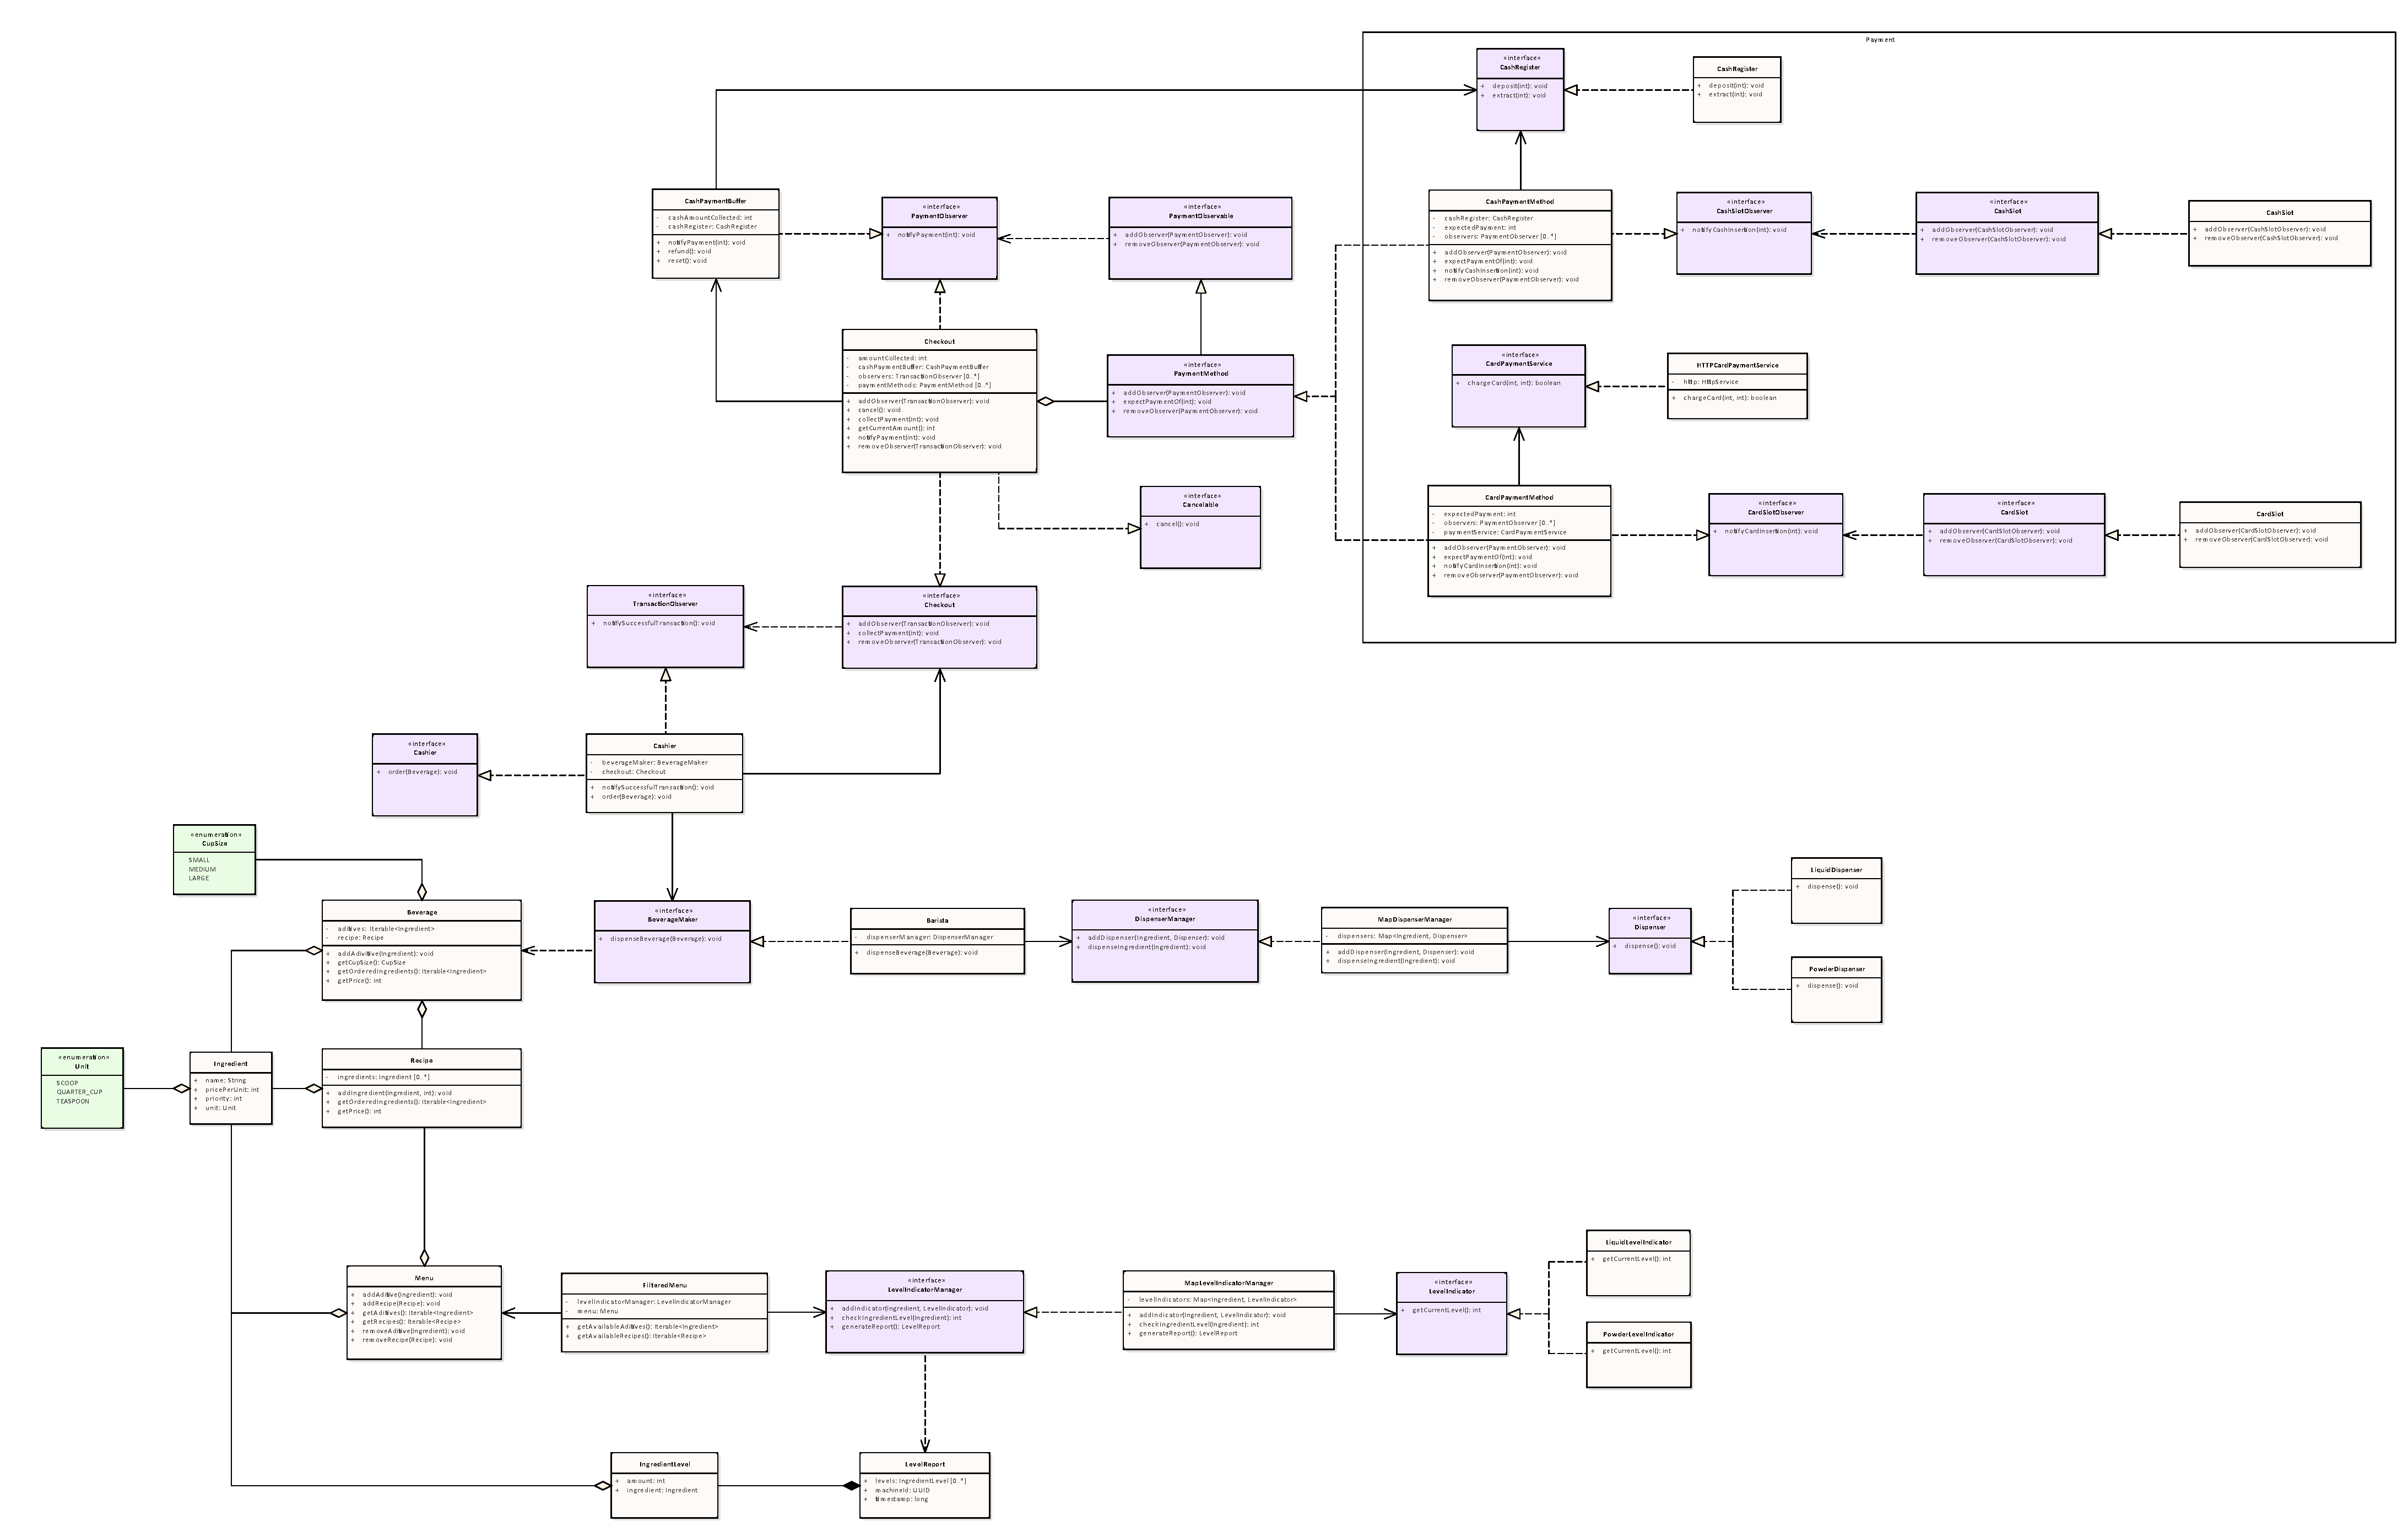
\includepdf[pages=-, scale=0.8, fitpaper, pagecommand={
        \subsection{Diagrama de clases de máquina de café}
        \thispagestyle{empty}
    }]{coffee-machine.pdf}

    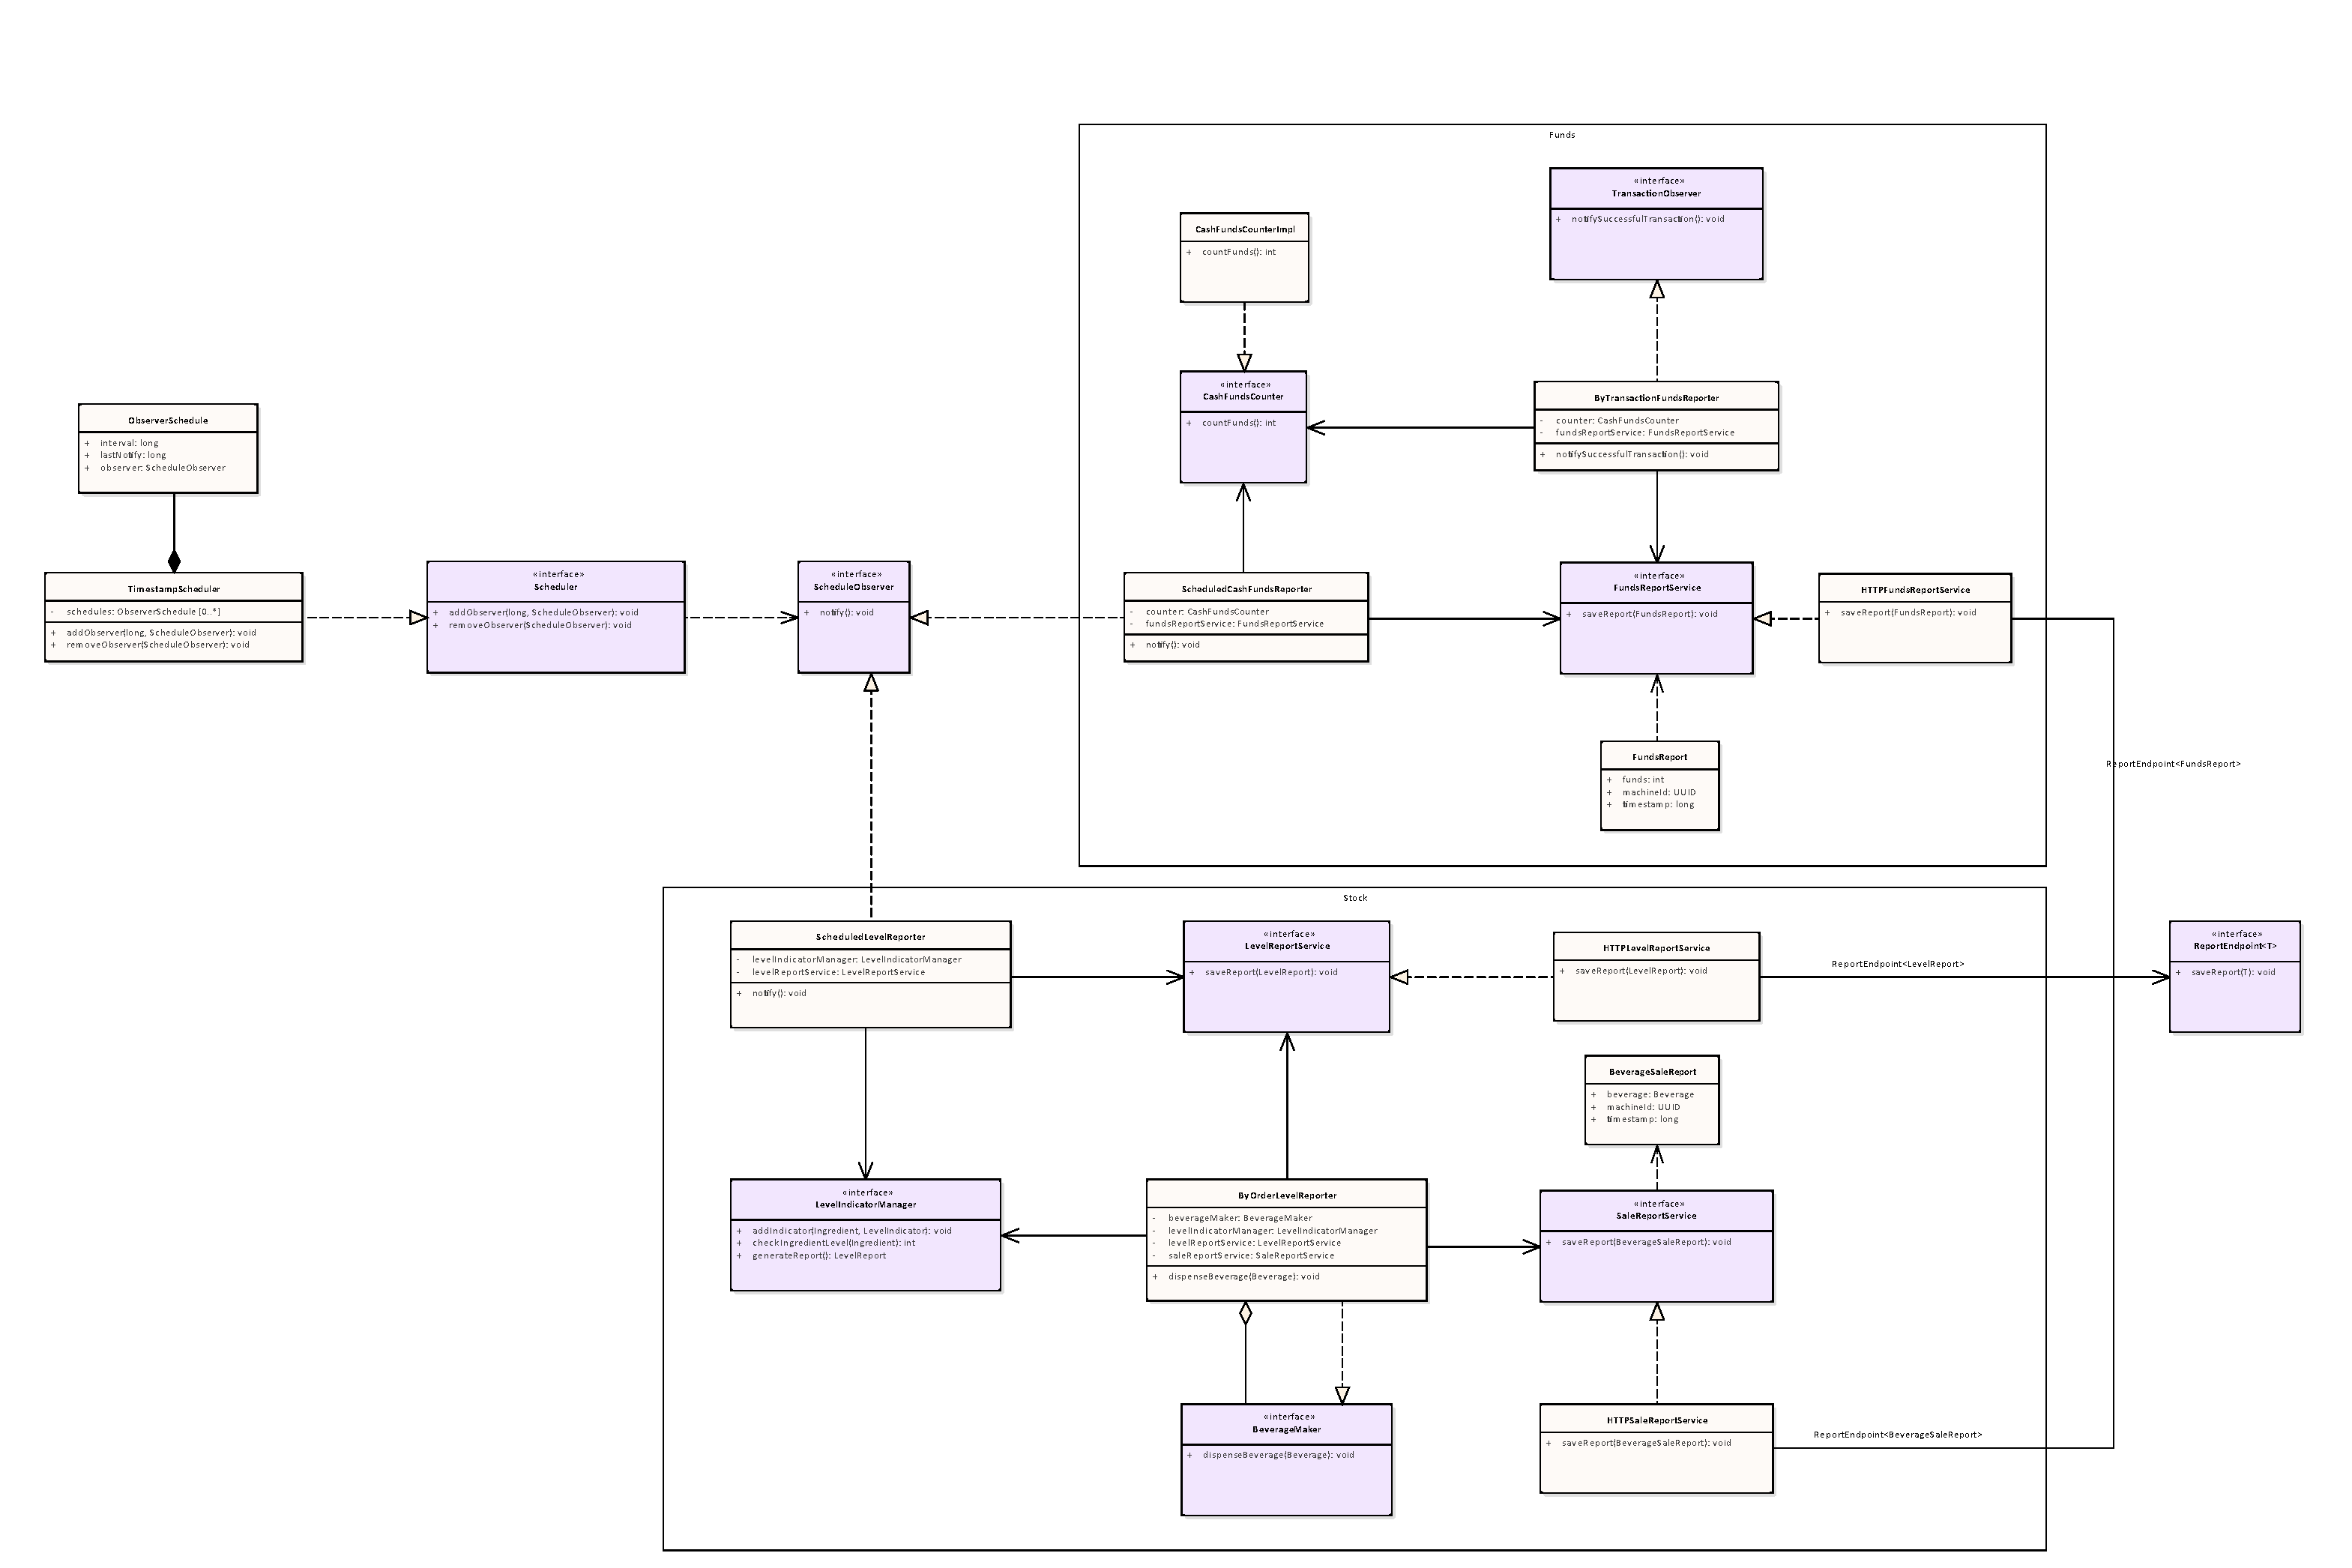
\includepdf[pages=-, scale=0.8, fitpaper, pagecommand={
        \thispagestyle{empty}
    }]{reports.pdf}

    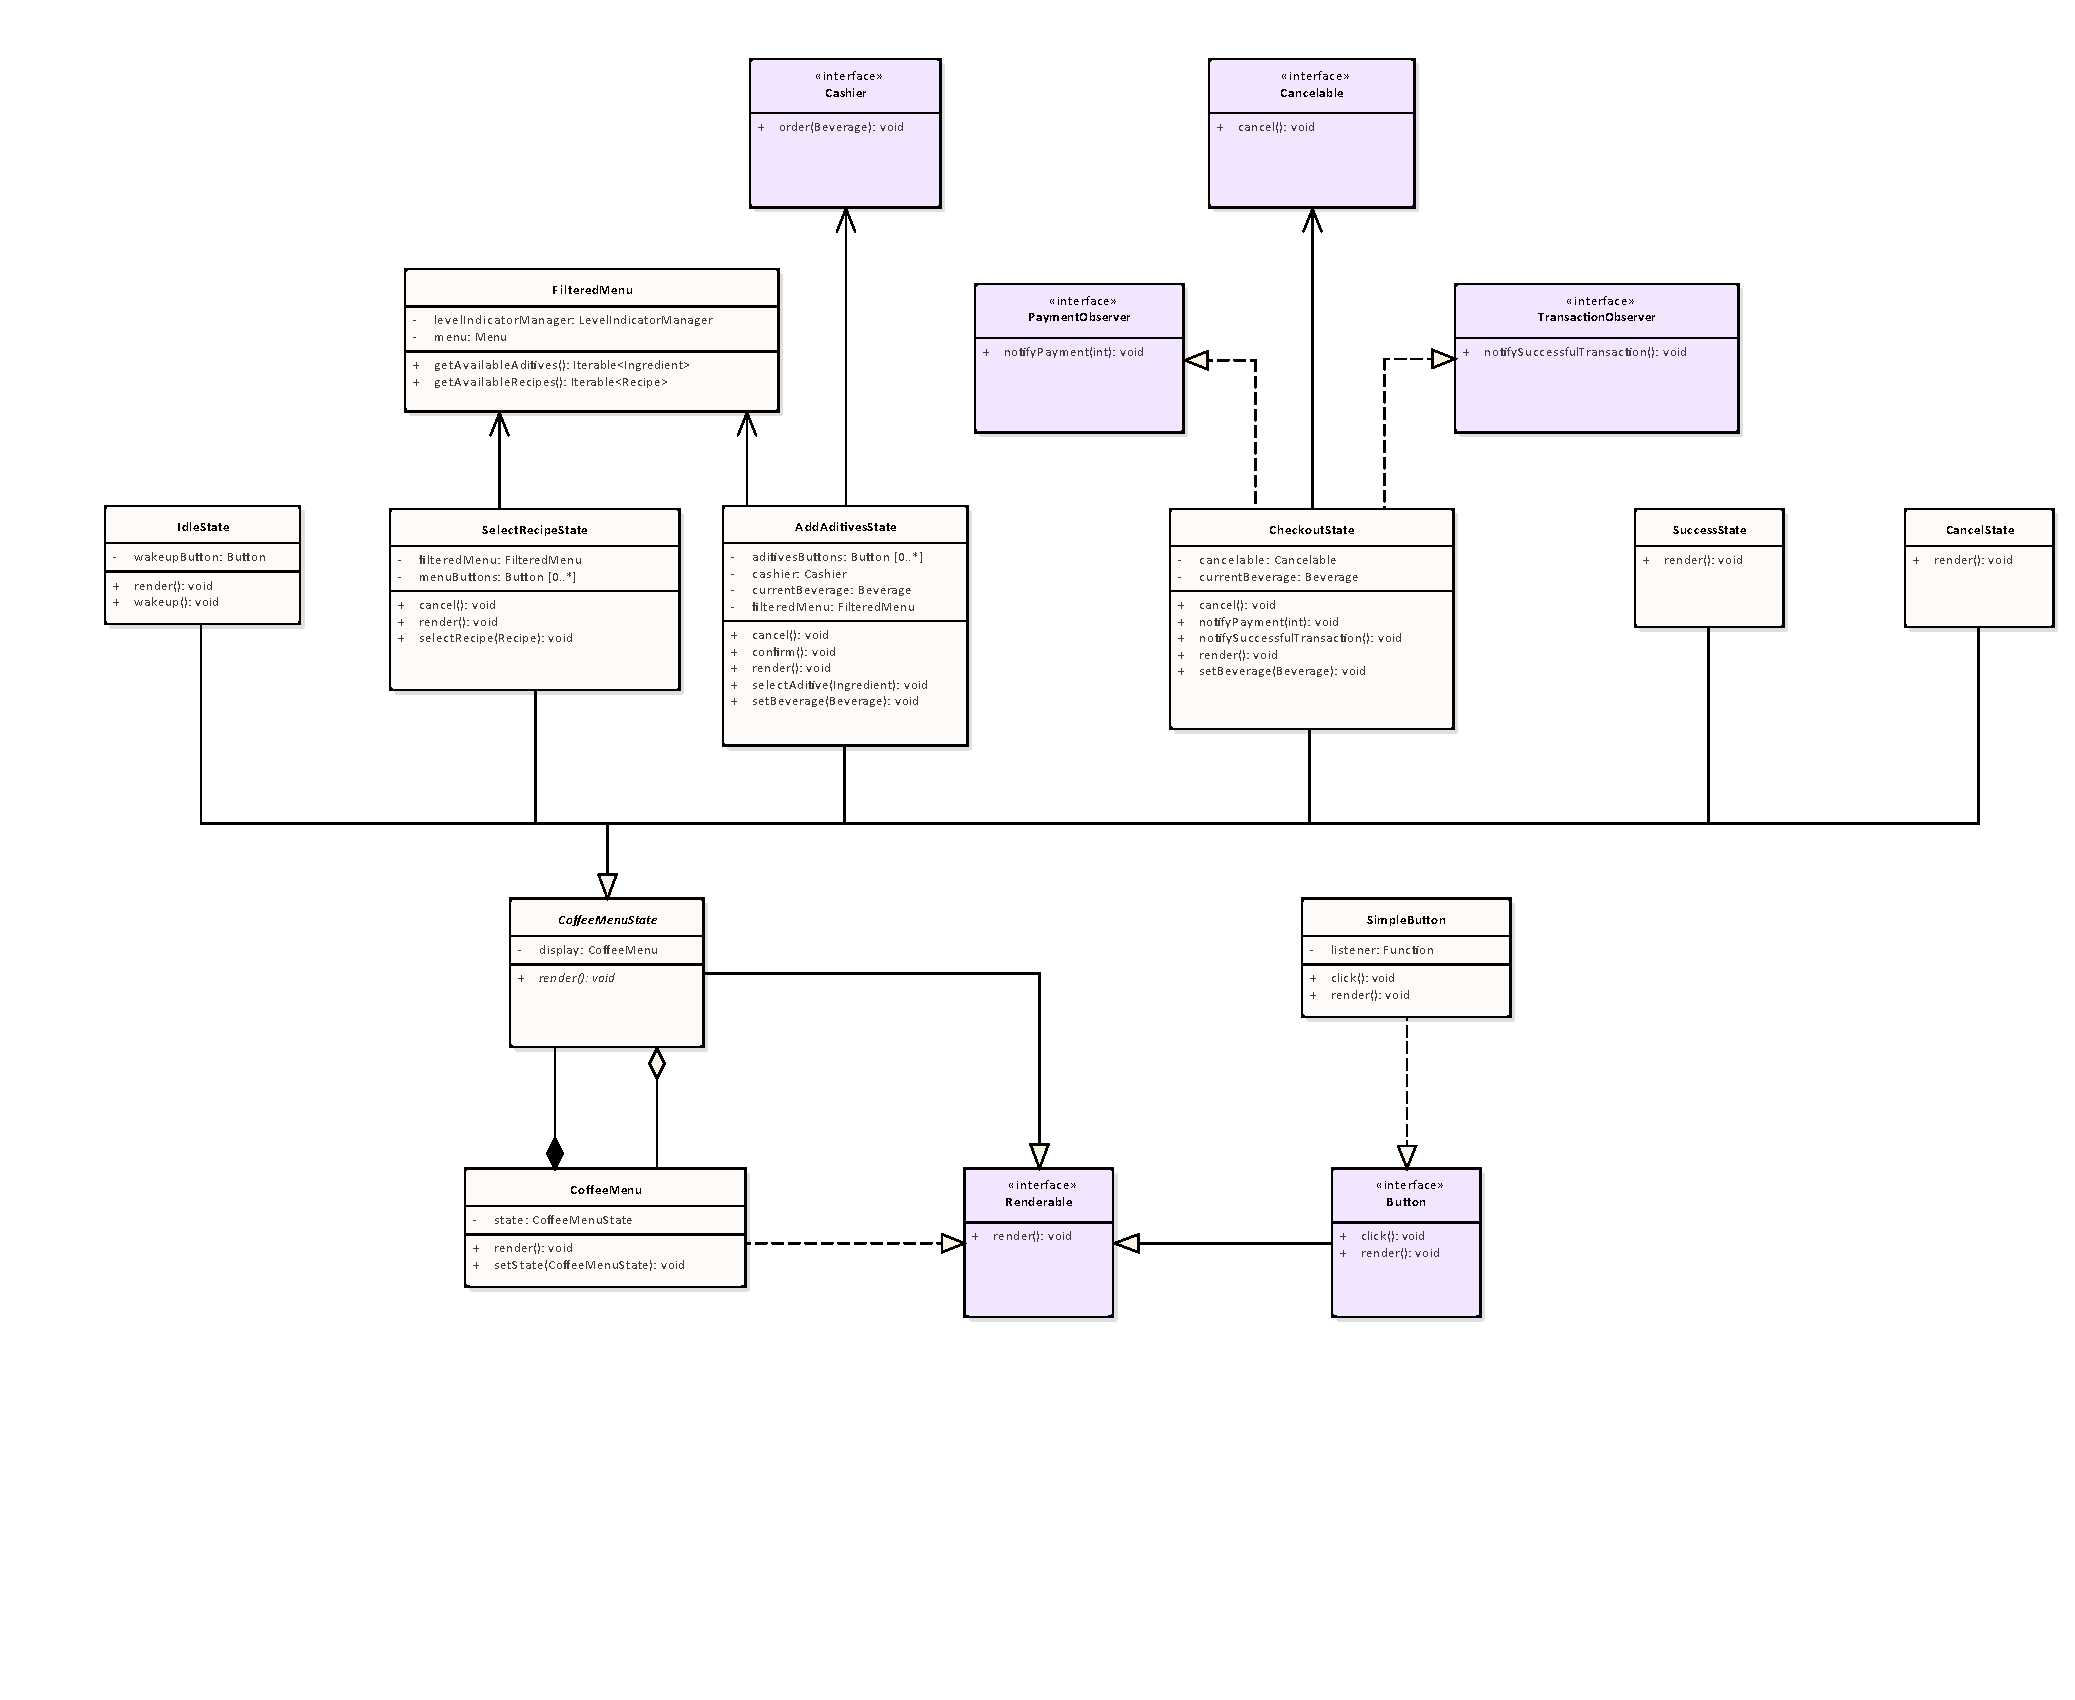
\includepdf[pages=-, scale=0.8, fitpaper, pagecommand={
        \thispagestyle{empty}
    }]{coffee-gui.pdf}

    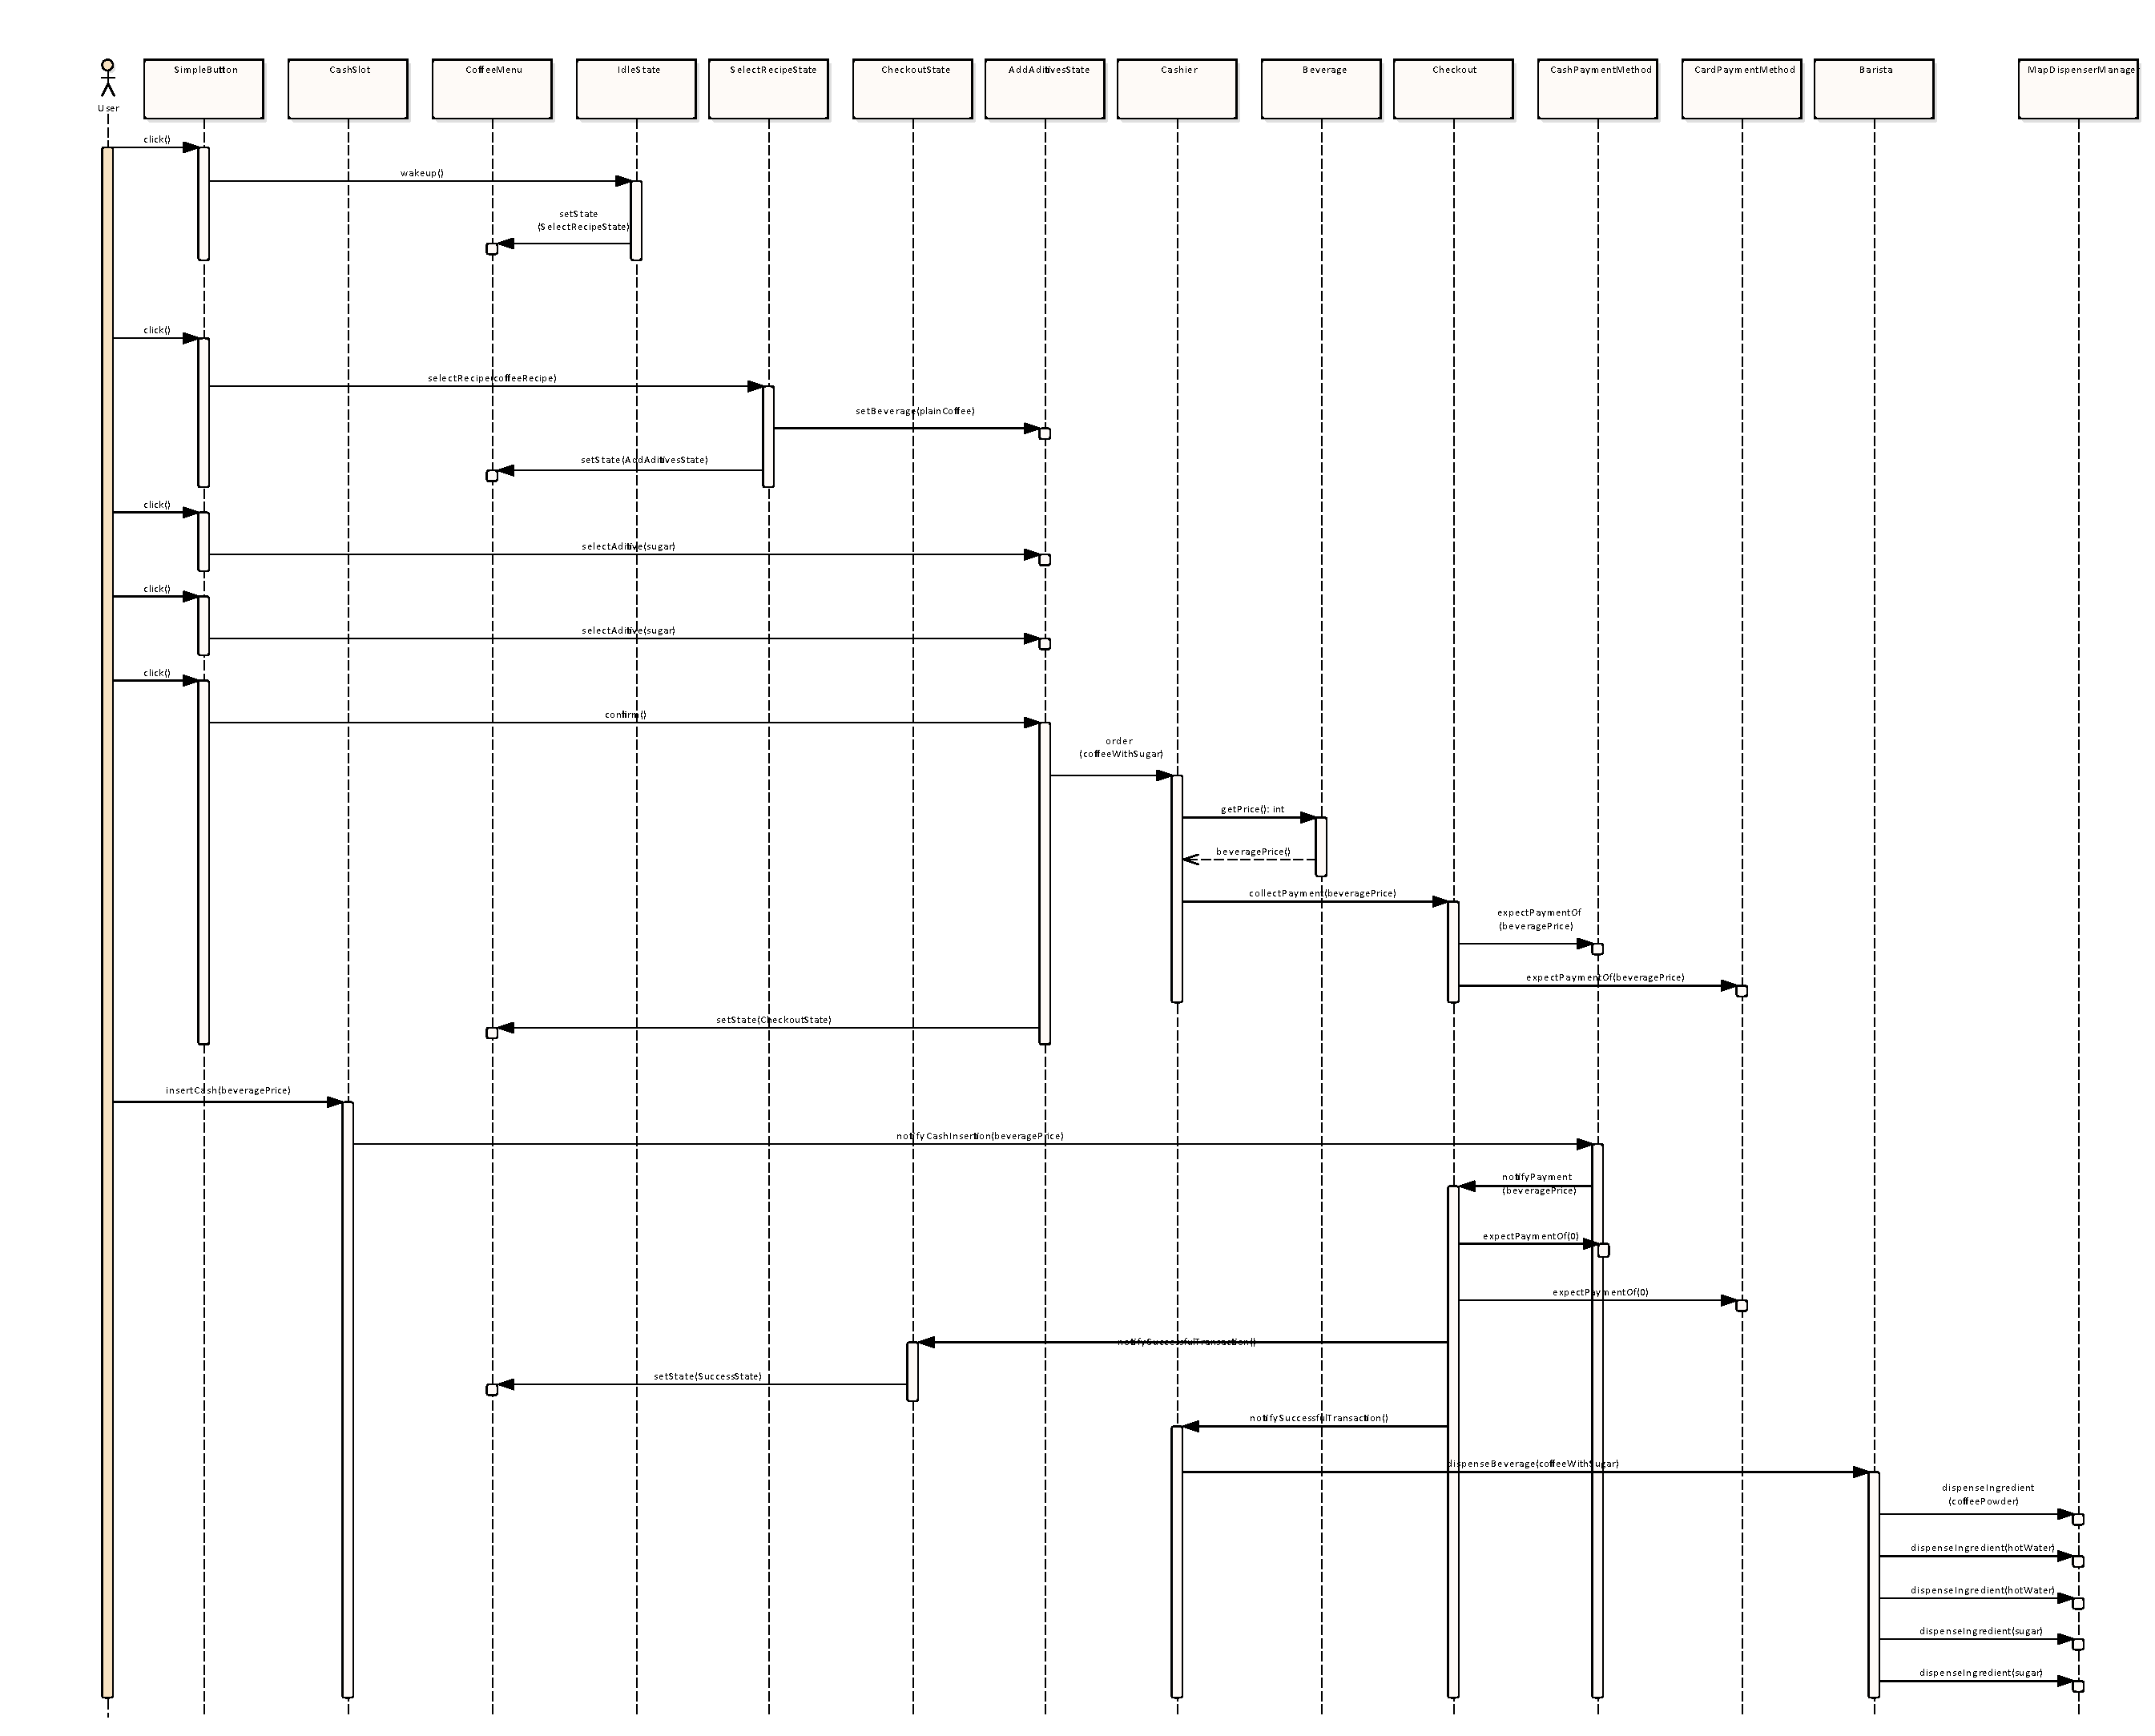
\includepdf[pages=-, scale=0.8, fitpaper, pagecommand={
        \subsection{Diagrama de secuencia de venta de café}
        \thispagestyle{empty}
    }]{order-coffee.pdf}

    \subsection{Caso de uso de control centralizado}
        \noindent\begin{tabularx}{\textwidth}{|l|l|l|}
            \cline{1-3}
            CU \textbf{001} & \multicolumn{2}{p{12cm}|}{MCU\_001\_Controldestock} \\ \cline{1-3}
            Versión & \multicolumn{2}{p{12cm}|}{1.0}  \\ \cline{1-3}
            Actores & \multicolumn{2}{p{12cm}|}{Administrador del sistema} \\ \cline{1-3}
            Referencias & \multicolumn{2}{p{12cm}|}{N/A} \\ \cline{1-3}
            Descripción & \multicolumn{2}{p{12cm}|}{Visualizar los reportes de stock y alarmas de reposición de todas las máquinas de café} \\ \cline{1-3}
            Precondiciones & \multicolumn{2}{p{12cm}|}{} \\ \cline{1-3}
            \multirow{3}{*}{Secuencia normal} & Paso & Descripción \\ \cline{2-3}
            &  & \\
            &  & \\
            &  & \\ \cline{1-3}
            Postcondición & \multicolumn{2}{p{12cm}|}{El administrador puede visualizar los reportes y alertas de reposición} \\ \cline{1-3}
            \multirow{3}{*}{Secuencia alternativa} & Paso & Descripción \\ \cline{2-3}
            & & \\
            & & \\
            & & \\ \cline{1-3}
            Comentarios & \multicolumn{2}{p{12cm}|}{} \\ \cline{1-3}
          \end{tabularx}

        
    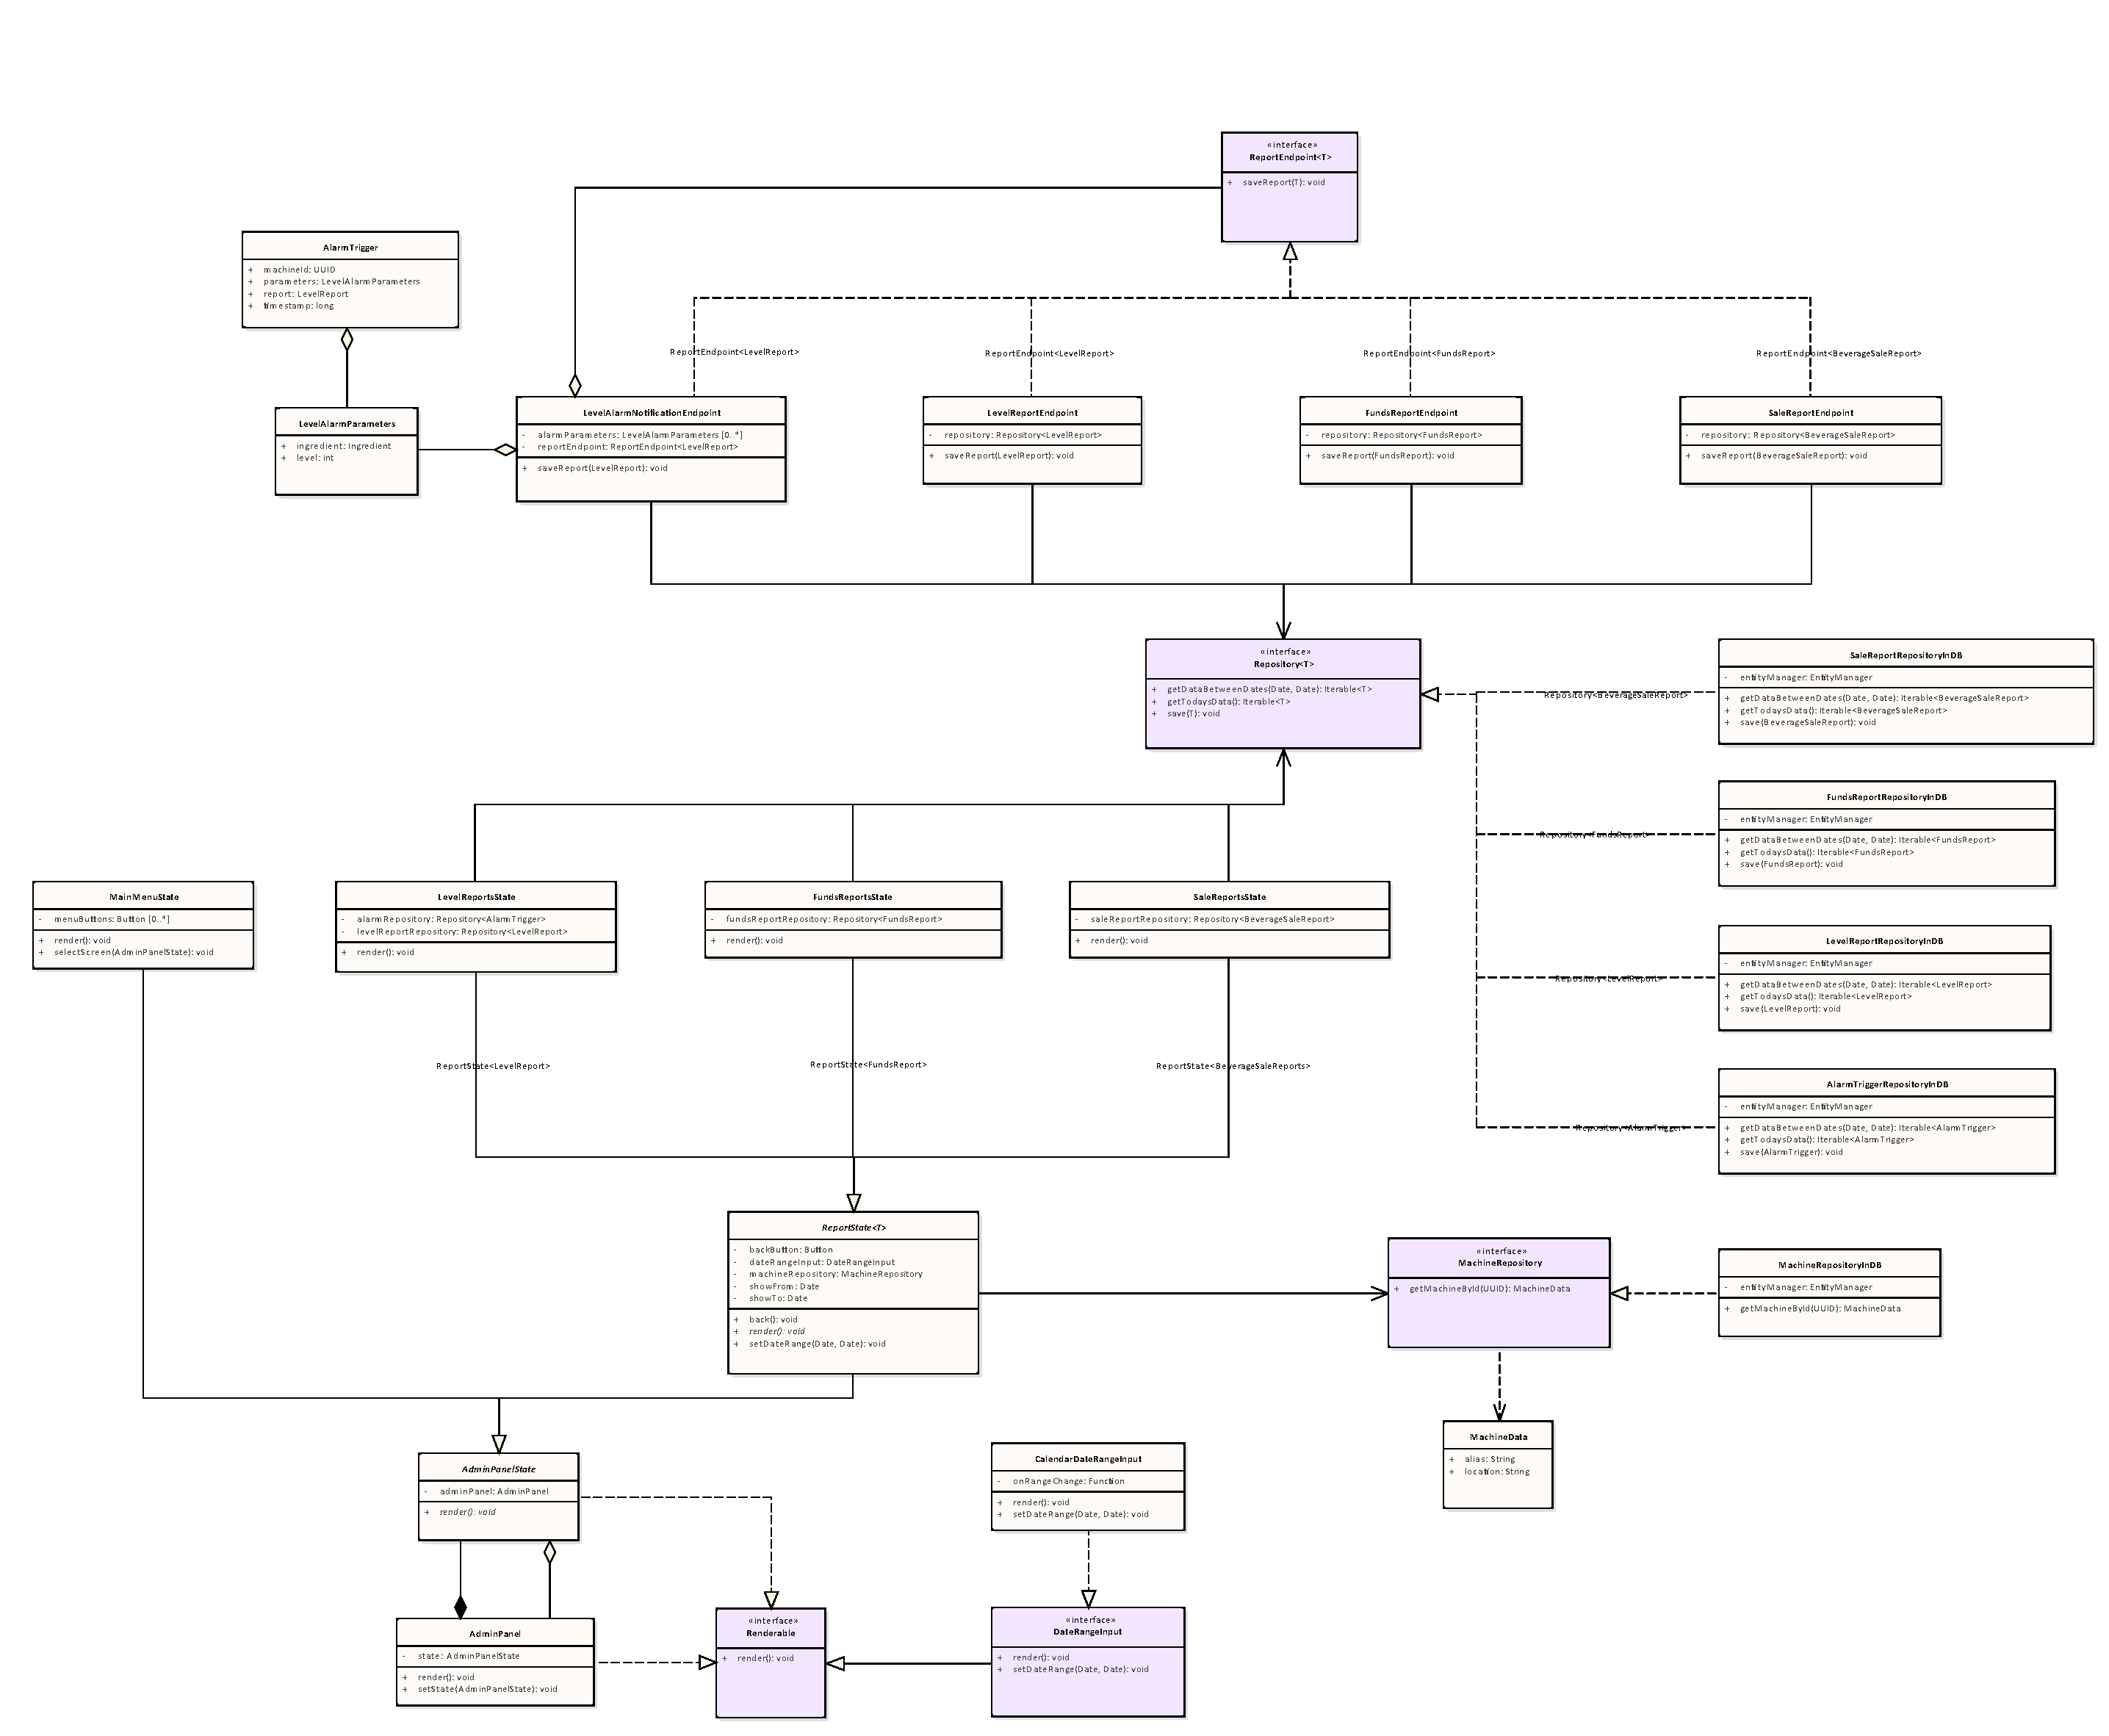
\includepdf[pages=-, fitpaper, scale=0.8, pagecommand={
        \subsection{Diagrama de clases de módulo central}
        \thispagestyle{empty}
    }]{central-module.pdf}

    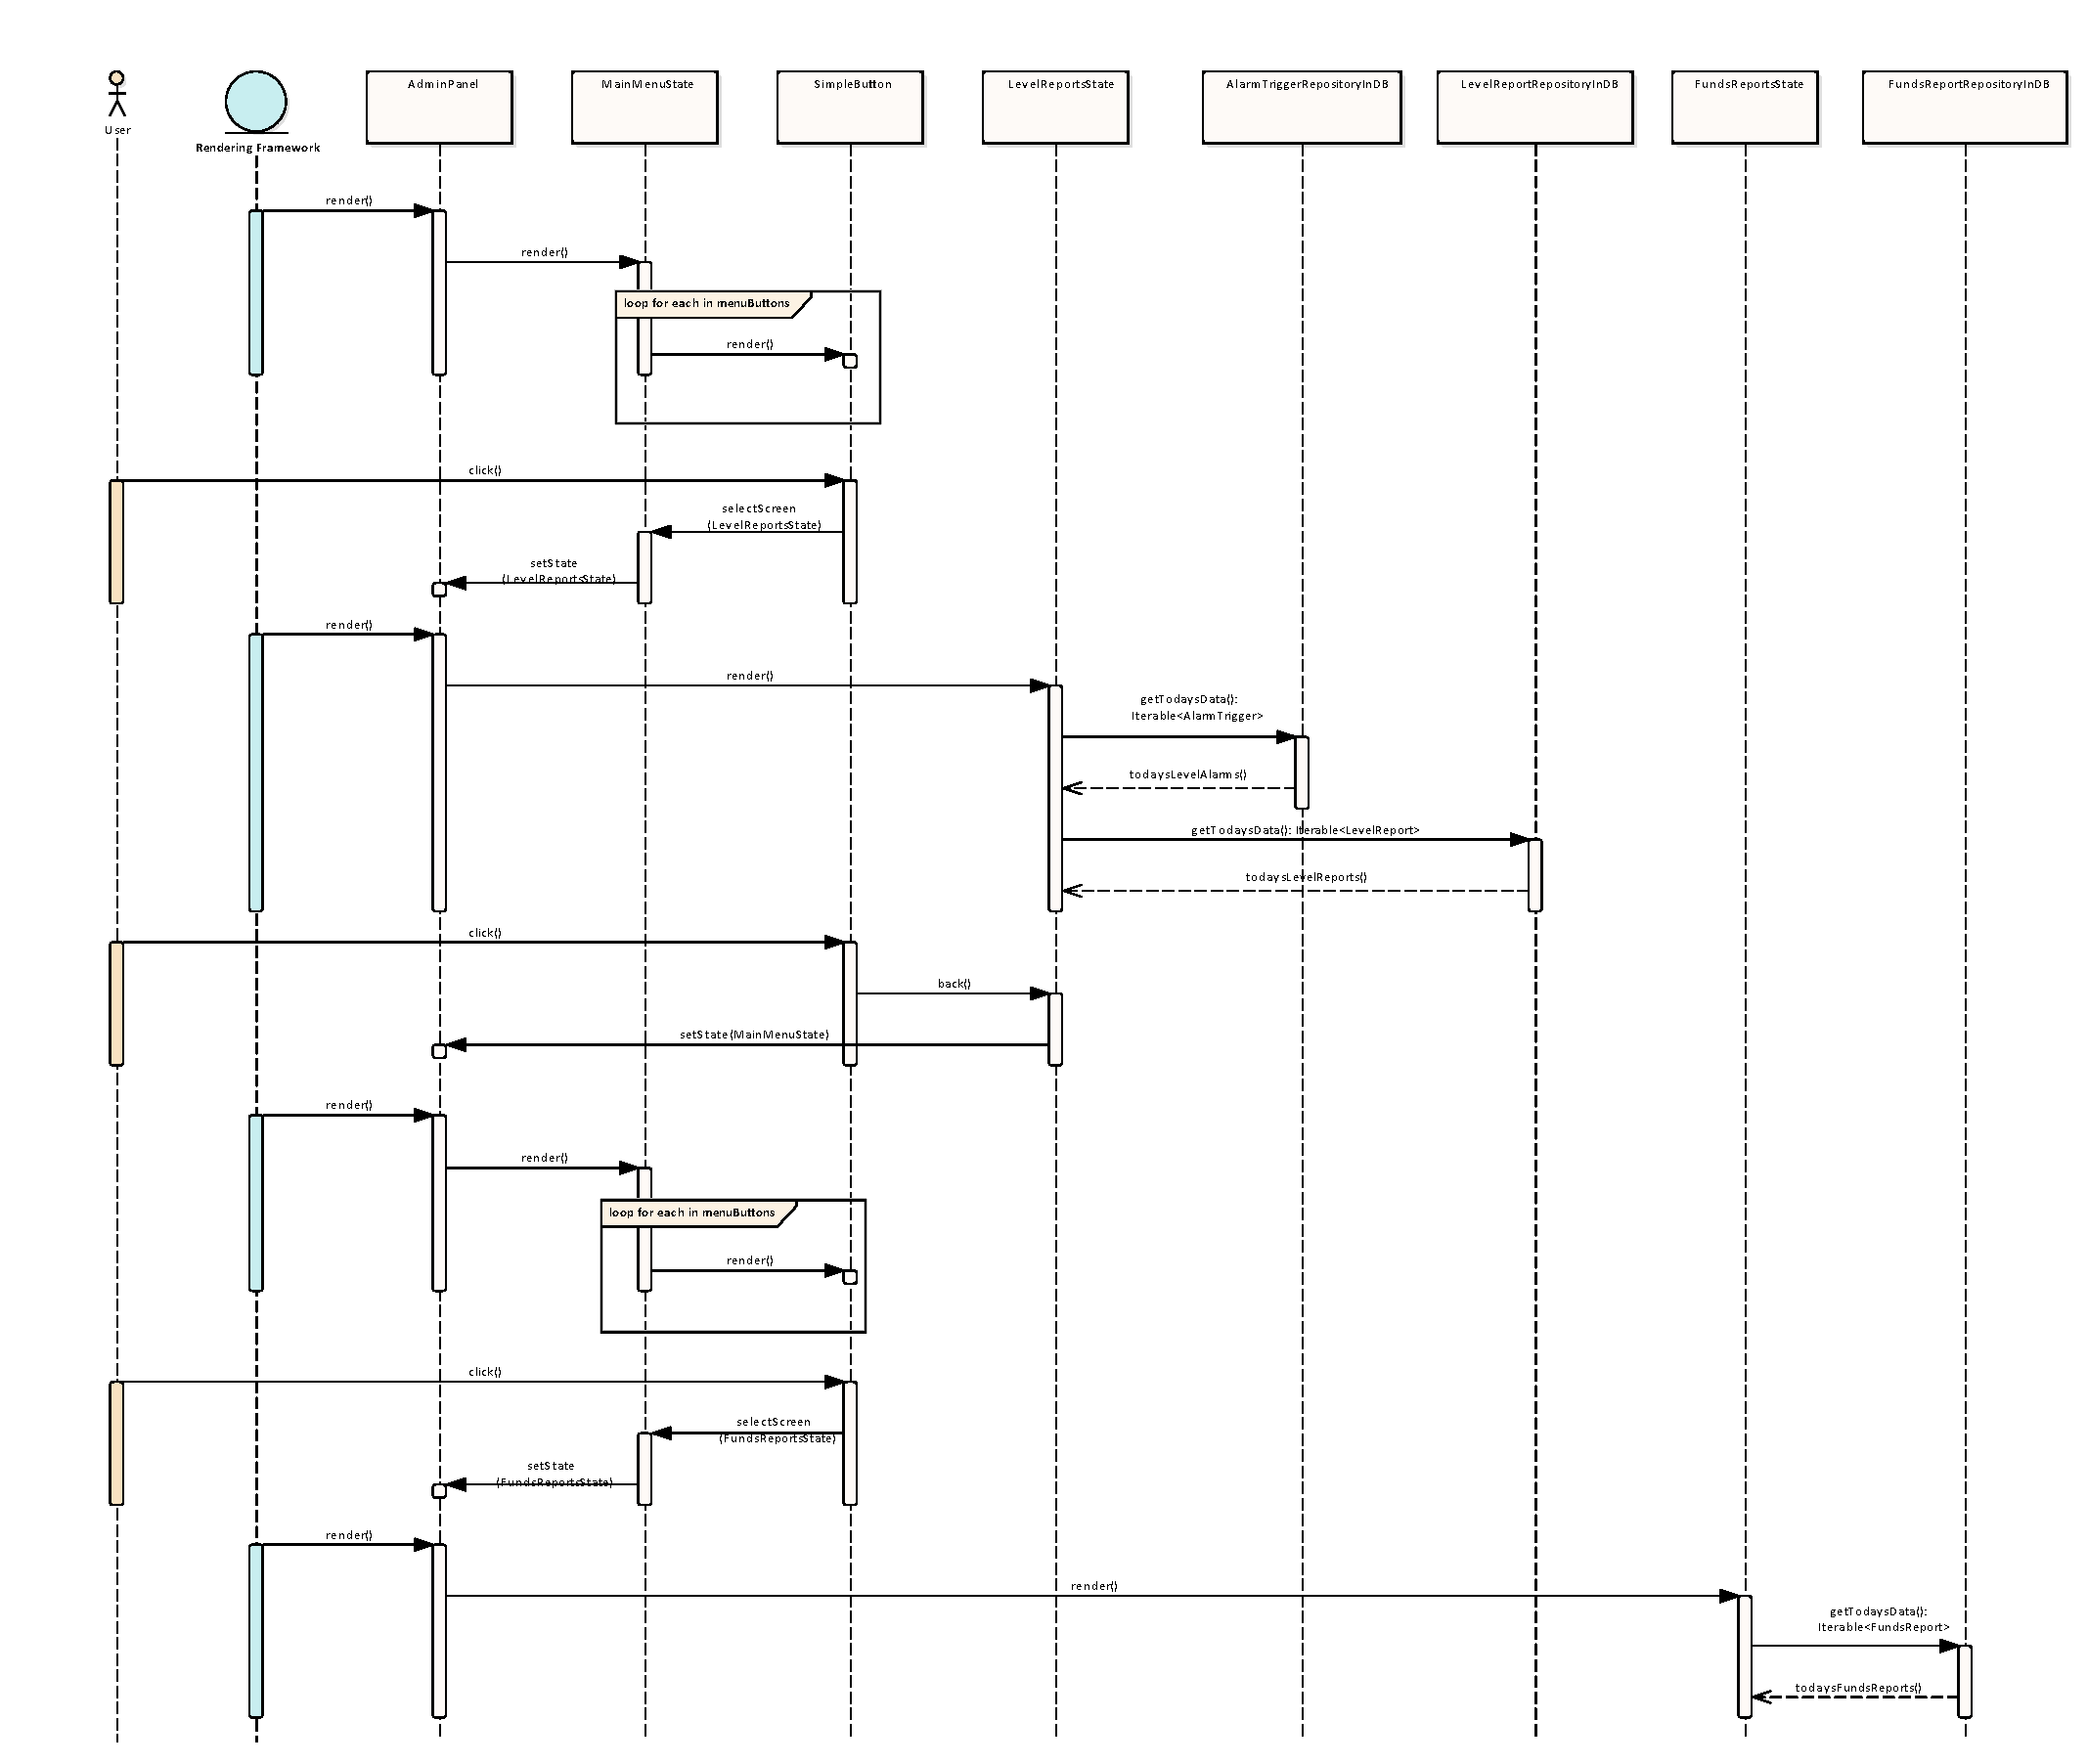
\includepdf[pages=-, fitpaper, scale=0.8, pagecommand={
        \subsection{Diagrama de secuencia de control centralizado}
        \thispagestyle{empty}
    }]{get-reports.pdf}

    
\end{document}
